\chapter{Конструкторская часть}


\section{Разработка алгоритмов}

На рисунках \ref{fig:standard_block} -  \ref{fig:vopt_block} приведены схемы алгоритмов, соотвтетственно, стандартного умножения матриц, умножения матриц по Винограду и оптимизированного умножения матриц по Винограду.

На схеме на рисунке \ref{fig:v_block} видно, что для алгоритма Винограда худшим случаем являются матрицы с нечётным общим размером, а лучшим - с чётным, так как отпадает необходимость в последнем цикле.

Алгоритм Винограда можно оптимизировать несколькими способами.
\begin{enumerate}[label={\arabic*)}]
	\item Заменить сравнение k < $\frac{n}{2}$ и инкремент k на сравнение k < n и прибавление 2 к k в заголовках циклов. При этом в телах циклов отпадает необходимость в умножении k на 2, а из n нужно заранее вычесть единицу, в последнем цикле изменить условие входа в него и убрать вычитание 1 из n.  
	\item Заменить все выражения вида a = a + с на a += с.
	\item Заменить в mulh += на -=, и тогда в третьем цикле  c[i][j] = mulh[i] - mulv[j].
\end{enumerate}


\begin{figure}[h!]
	
	\centering{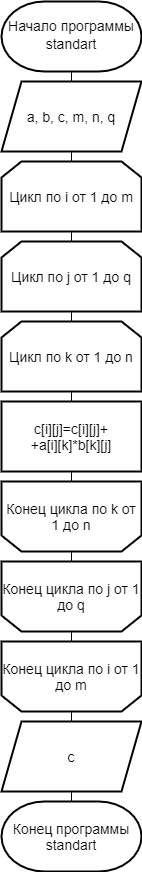
\includegraphics[scale=0.7]{inc/img/standard_block.png}}
	
	\caption{Стандартный алгоритм умножения матриц}
	
	\label{fig:standard_block}
	
\end{figure}


\begin{figure}[h!]
	
	\centering{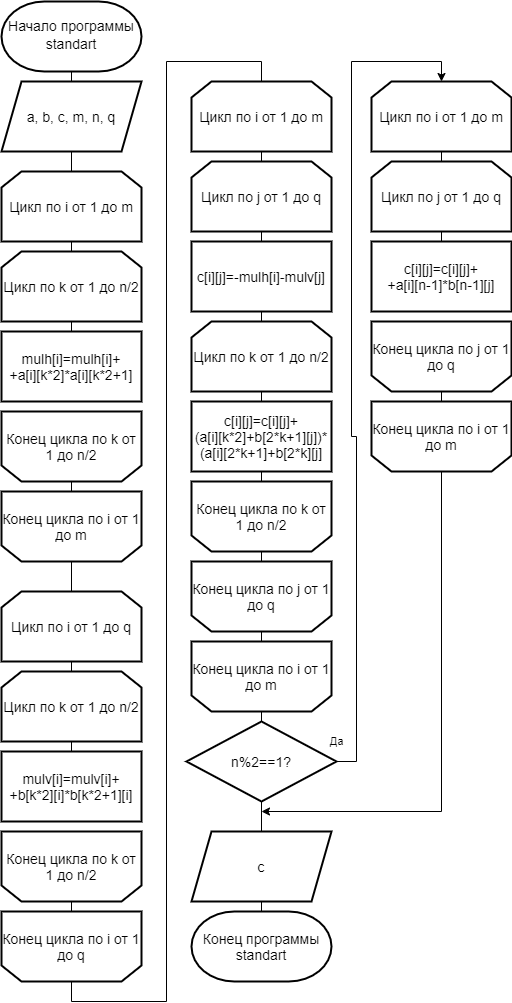
\includegraphics[scale=0.7]{inc/img/v_block.png}}
		
	\caption{Алгоритм умножения матриц по Винограду}
		
	\label{fig:v_block}
		
\end{figure}


\begin{figure}[h!]
	
	\centering{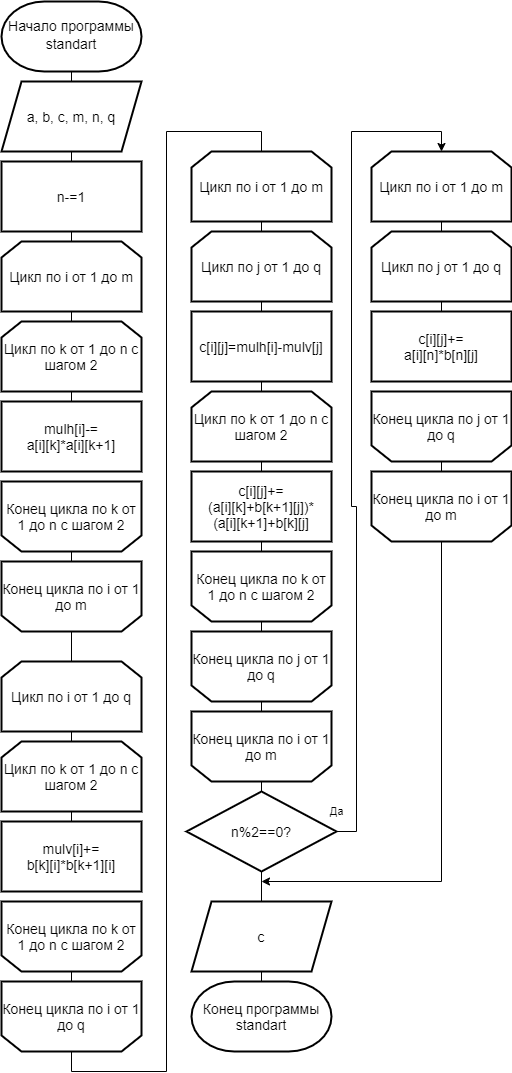
\includegraphics[scale=0.65]{inc/img/vopt_block.png}}
		
	\caption{Оптимизированный алгоритм умножения матриц по Винограду}
		
	\label{fig:vopt_block}
		
\end{figure}

\section{Оценка трудоемкости}

Произведем теоретическую оценку трудоемкости алгоритмов умножения матриц.

\begin{enumerate}
	\item Стандартный алгоритм:
	$$f=2+m(2+2+q(2+2+n(2+8+1+1+1*2)))=14mnq+4mq+4m+2$$

	\item Алгоритм Винограда, складывающийся из 4 циклов:
	$$f1=2+m(2+4+\frac{n}{2}(4+6+1+2+3*2))=\frac{19}{2}mn+6m+2$$
	
	$$f2=2+q(2+4+\frac{n}{2}(4+6+1+2+3*2))=\frac{19}{2}qn+6q+2$$
	
	$$f3=2+m(2+2+q(2+7+4+\frac{n}{2}(4+1+12+5+5*2)))=16mnq+13mq+4m+2$$
	
	$$f4=3+
	\left[ 
	\begin{array}{c} 
		$0, л.с. (n четное)$\\
		$2+m(2+2+q(2+8+1+3+1*2))=16mq+4m+2, х.с.$
	\end{array}
	\right.\\$$
	Итоговая трудоемкость - сумма трудоемкостей каждого цикла:
	
	$$f=16mnq+13mq+\frac{19}{2} mn+\frac{19}{2} qn+10m+6q+9+
	\left[ 
\begin{array}{c} 
	$0, л.с. (n четное)$\\
	$16mq+4m+2, х.с.$
\end{array}
\right.\\$$

Трудоемкость выше по сравнению со стандартной из-за отсутствия оптимизаций.
	

	\item Оптимизированный алгоритм Винограда расчитывается аналогично, не упуская при этом вычитание из n единицы в самом начале:
	
	$$f1=1+2+m(2+2+\frac{n}{2}(2+5+2+1*2))=\frac{11}{2}mn+4m+3$$

	$$f2=2+q(2+2+\frac{n}{2}(2+5+2+1*2))=\frac{11}{2}qn+4q+2$$

	$$f3=2+m(2+2+q(2+6+2+\frac{n}{2}(2+1+10+4+1*2)))=\frac{19}{2}mnq+10mq+4m+2$$

$$f4=3+
\left[ 
\begin{array}{c} 
	$0, л.с. (n четное)$\\
	$2+m(2+2+q(2+6+1+1*2))=13mq+4m+2, х.с.$
\end{array}
\right.\\$$

$$f=\frac{19}{2}mnq+10mq+\frac{11}{2} mn+\frac{11}{2} qn+8m+4q+10+
\left[ 
\begin{array}{c} 
	$0, л.с. (n четное)$\\
	$13mq+4m+2, х.с.$
\end{array}
\right.\\$$
	Трудоемкость меньше по сравнению со стандартным алгоритмом за счет меньшей доли умножений. 
\end{enumerate}


\section*{Вывод}

Были разработаны схемы алгоритмов, позволяющих с помощью различных подходов находить произведение матриц, а также была дана оценка их трудоемкости.


